
\documentclass[11pt,a4paper]{article}
\usepackage[margin=1in]{geometry}
\usepackage{amsmath,amssymb,amsfonts}
\usepackage{tikz}
\usetikzlibrary{positioning,arrows.meta,shapes.geometric,fit,calc,backgrounds,decorations.pathreplacing}
\usepackage{xcolor}
\usepackage{hyperref}
\usepackage{booktabs}

\definecolor{embed}{RGB}{66,133,244}
\definecolor{attn}{RGB}{234,67,53}
\definecolor{mlp}{RGB}{251,188,4}
\definecolor{norm}{RGB}{52,168,83}
\definecolor{cond}{RGB}{153,0,255}
\definecolor{residual}{RGB}{100,100,100}
\definecolor{mask}{RGB}{255,109,0}

\title{Architecture of DDiT and ContDIT\\[0.5em]\large From High-Level Overview to Full Mathematical Detail}
\author{Auto-generated from CANDI Diffusion Codebase}
\date{\today}

\begin{document}
\maketitle
\tableofcontents
\newpage

%% ============================================================
%% SECTION 1: HIGH-LEVEL OVERVIEW
%% ============================================================
\section{Level 1: High-Level Overview}

Both DDiT and ContDIT are \textbf{Diffusion Transformers} for discrete text generation.
They share the same internal transformer block structure but differ in how inputs are prepared and what noise processes they handle.

\subsection{DDiT --- Discrete Diffusion Transformer}

DDiT operates on sequences corrupted by \textbf{discrete masking} only. It takes token IDs and a scalar noise level $\sigma$, and predicts logits over the vocabulary.

\begin{center}
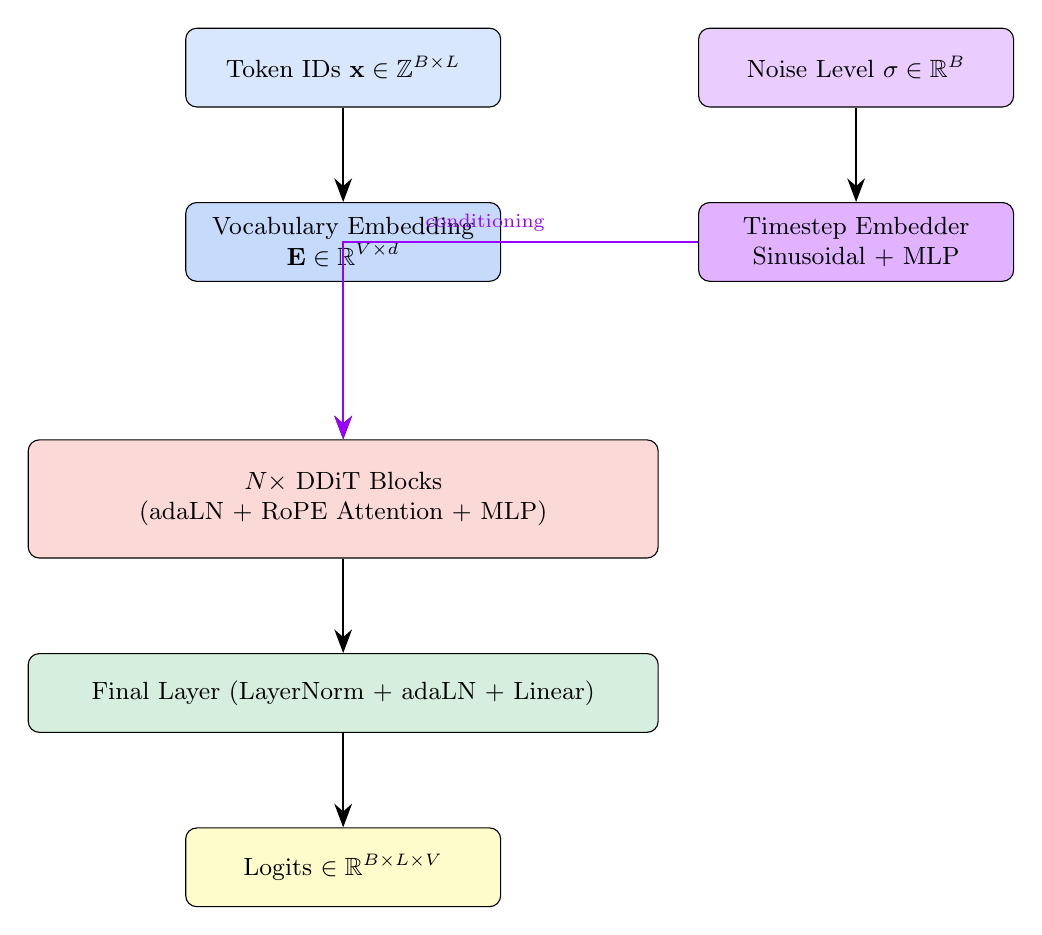
\begin{tikzpicture}[
    block/.style={draw, rounded corners, minimum width=4cm, minimum height=1cm, align=center, font=\small},
    arrow/.style={-{Stealth[length=3mm]}, thick},
    node distance=1.2cm
]
    % Input
    \node[block, fill=embed!20] (input) {Token IDs $\mathbf{x} \in \mathbb{Z}^{B \times L}$};
    \node[block, fill=cond!20, right=2.5cm of input] (sigma) {Noise Level $\sigma \in \mathbb{R}^B$};
    
    % Embedding
    \node[block, fill=embed!30, below=of input] (embed) {Vocabulary Embedding\\$\mathbf{E} \in \mathbb{R}^{V \times d}$};
    
    % Timestep
    \node[block, fill=cond!30, below=of sigma] (tsemb) {Timestep Embedder\\Sinusoidal + MLP};
    
    % Transformer
    \node[block, fill=attn!20, below=2cm of embed, minimum width=8cm, minimum height=1.5cm] (transformer) {$N \times$ DDiT Blocks\\(adaLN + RoPE Attention + MLP)};
    
    % Output
    \node[block, fill=norm!20, below=of transformer, minimum width=8cm] (final) {Final Layer (LayerNorm + adaLN + Linear)};
    
    % Logits
    \node[block, fill=yellow!20, below=of final, minimum width=4cm] (logits) {Logits $\in \mathbb{R}^{B \times L \times V}$};
    
    % Arrows
    \draw[arrow] (input) -- (embed);
    \draw[arrow] (sigma) -- (tsemb);
    \draw[arrow] (embed) -- (transformer);
    \draw[arrow, color=cond] (tsemb) -| node[above, pos=0.3, font=\scriptsize, color=cond]{conditioning} (transformer);
    \draw[arrow] (transformer) -- (final);
    \draw[arrow] (final) -- (logits);
\end{tikzpicture}
\end{center}

\subsection{ContDIT --- Continuous + Discrete Diffusion Transformer}

ContDIT handles CANDI's \textbf{hybrid noise process}: tokens are corrupted by both discrete masking \textbf{and} continuous Gaussian noise in embedding space.

\begin{center}
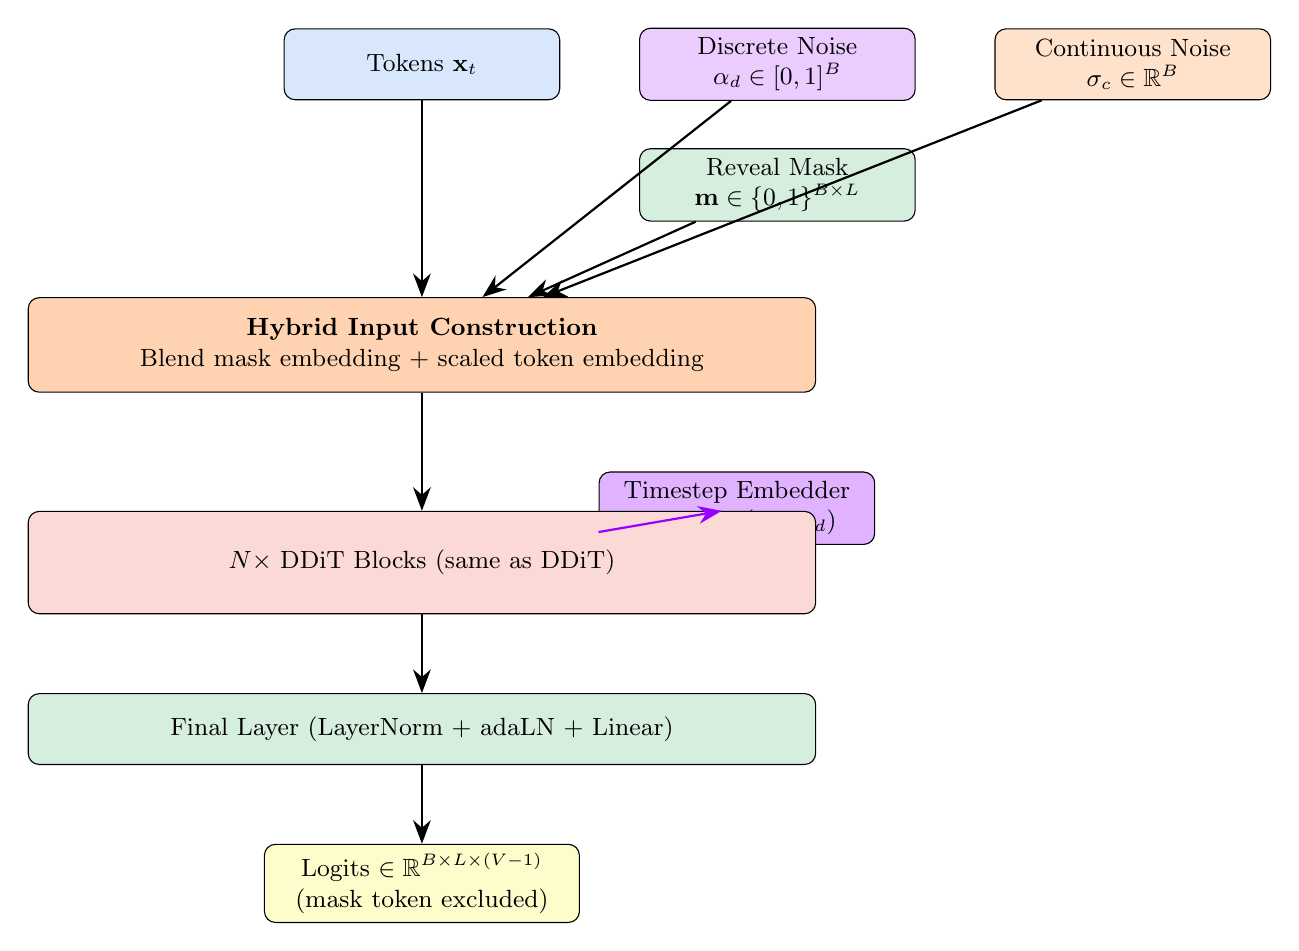
\begin{tikzpicture}[
    block/.style={draw, rounded corners, minimum width=3.5cm, minimum height=0.9cm, align=center, font=\small},
    arrow/.style={-{Stealth[length=3mm]}, thick},
    node distance=1.0cm
]
    % Inputs
    \node[block, fill=embed!20] (xt) {Tokens $\mathbf{x}_t$};
    \node[block, fill=cond!20, right=1cm of xt] (dn) {Discrete Noise\\$\alpha_d \in [0,1]^B$};
    \node[block, fill=mask!20, right=1cm of dn] (cn) {Continuous Noise\\$\sigma_c \in \mathbb{R}^B$};
    \node[block, fill=norm!20, below=0.6cm of dn] (rm) {Reveal Mask\\$\mathbf{m} \in \{0,1\}^{B \times L}$};
    
    % Hybrid Input Construction
    \node[block, fill=mask!30, below=2.5cm of xt, minimum width=10cm, minimum height=1.2cm] (hybrid) {\textbf{Hybrid Input Construction}\\Blend mask embedding + scaled token embedding};
    
    % Timestep
    \node[block, fill=cond!30, below=of hybrid, xshift=4cm] (tsemb2) {Timestep Embedder\\$\sigma = -\log(1-\alpha_d)$};
    
    % Transformer
    \node[block, fill=attn!20, below=1.5cm of hybrid, minimum width=10cm, minimum height=1.3cm, xshift=0cm] (transformer2) {$N \times$ DDiT Blocks (same as DDiT)};
    
    % Output
    \node[block, fill=norm!20, below=of transformer2, minimum width=10cm] (final2) {Final Layer (LayerNorm + adaLN + Linear)};
    
    % Logits
    \node[block, fill=yellow!20, below=of final2, minimum width=4cm] (logits2) {Logits $\in \mathbb{R}^{B \times L \times (V{-}1)}$\\(mask token excluded)};
    
    % Arrows
    \draw[arrow] (xt) -- (hybrid);
    \draw[arrow] (dn) -- (hybrid);
    \draw[arrow] (cn) -- (hybrid);
    \draw[arrow] (rm) -- (hybrid);
    \draw[arrow] (hybrid) -- (transformer2);
    \draw[arrow, color=cond] (tsemb2) -- (transformer2);
    \draw[arrow] (transformer2) -- (final2);
    \draw[arrow] (final2) -- (logits2);
\end{tikzpicture}
\end{center}

\newpage

%% ============================================================
%% SECTION 2: DDiT BLOCK INTERNALS
%% ============================================================
\section{Level 2: DDiT Block Internals}

Each DDiT Block consists of two sub-layers: \textbf{Multi-Head Self-Attention} (with RoPE) and a \textbf{Feed-Forward Network} (MLP), both conditioned via \textbf{Adaptive Layer Normalization} (adaLN).

\subsection{DDiT Block with adaLN}

\begin{center}
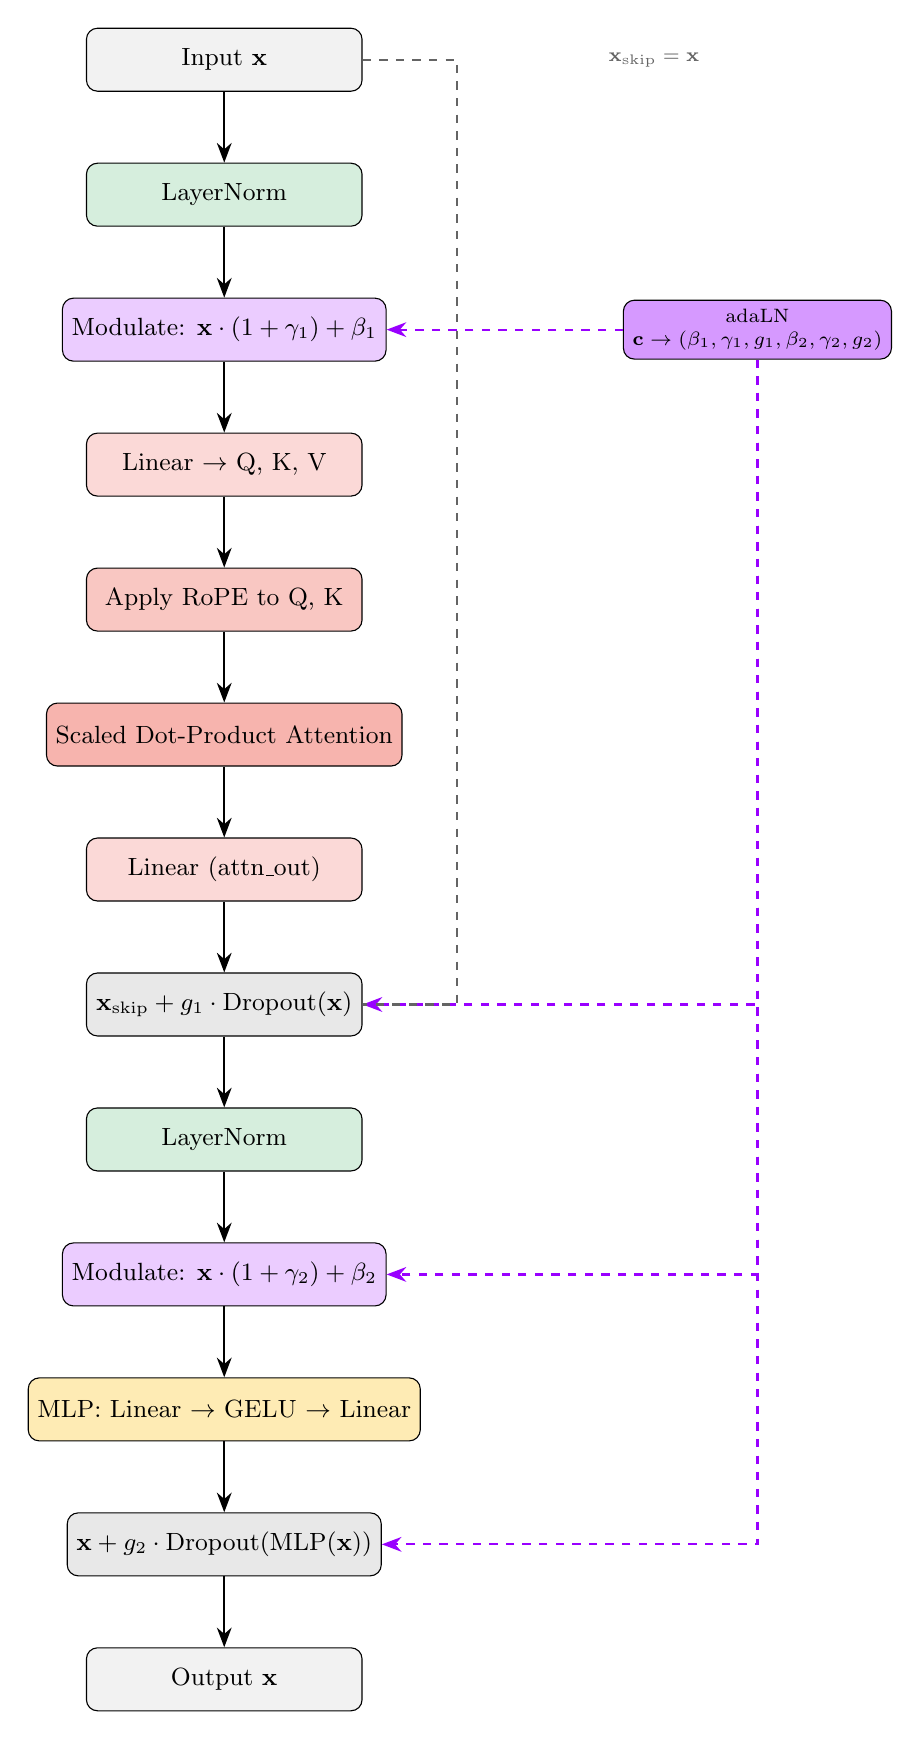
\begin{tikzpicture}[
    block/.style={draw, rounded corners, minimum width=3.5cm, minimum height=0.8cm, align=center, font=\small},
    smallblock/.style={draw, rounded corners, minimum width=2.5cm, minimum height=0.6cm, align=center, font=\scriptsize},
    arrow/.style={-{Stealth[length=2.5mm]}, thick},
    dasharrow/.style={-{Stealth[length=2.5mm]}, thick, dashed, color=cond},
    node distance=0.9cm
]
    % Input
    \node[block, fill=gray!10] (xin) {Input $\mathbf{x}$};
    
    % Save residual
    \node[font=\scriptsize, right=3cm of xin, color=residual] (skip1) {$\mathbf{x}_{\text{skip}} = \mathbf{x}$};
    
    % LayerNorm 1
    \node[block, fill=norm!20, below=of xin] (ln1) {LayerNorm};
    
    % adaLN modulate 1
    \node[block, fill=cond!20, below=of ln1] (mod1) {Modulate: $\mathbf{x} \cdot (1 + \gamma_1) + \beta_1$};
    
    % Conditioning source
    \node[smallblock, fill=cond!40, right=3cm of mod1] (adaln) {adaLN\\$\mathbf{c} \to (\beta_1, \gamma_1, g_1, \beta_2, \gamma_2, g_2)$};
    
    % QKV
    \node[block, fill=attn!20, below=of mod1] (qkv) {Linear $\to$ Q, K, V};
    
    % RoPE
    \node[block, fill=attn!30, below=of qkv] (rope) {Apply RoPE to Q, K};
    
    % Attention
    \node[block, fill=attn!40, below=of rope] (attn) {Scaled Dot-Product Attention};
    
    % Output projection
    \node[block, fill=attn!20, below=of attn] (out1) {Linear (attn\_out)};
    
    % Gate + residual 1
    \node[block, fill=residual!15, below=of out1] (res1) {$\mathbf{x}_{\text{skip}} + g_1 \cdot \text{Dropout}(\mathbf{x})$};
    
    % LayerNorm 2
    \node[block, fill=norm!20, below=of res1] (ln2) {LayerNorm};
    
    % adaLN modulate 2
    \node[block, fill=cond!20, below=of ln2] (mod2) {Modulate: $\mathbf{x} \cdot (1 + \gamma_2) + \beta_2$};
    
    % MLP
    \node[block, fill=mlp!30, below=of mod2] (mlp) {MLP: Linear $\to$ GELU $\to$ Linear};
    
    % Gate + residual 2
    \node[block, fill=residual!15, below=of mlp] (res2) {$\mathbf{x} + g_2 \cdot \text{Dropout}(\text{MLP}(\mathbf{x}))$};
    
    % Output
    \node[block, fill=gray!10, below=of res2] (xout) {Output $\mathbf{x}$};
    
    % Arrows
    \draw[arrow] (xin) -- (ln1);
    \draw[arrow] (ln1) -- (mod1);
    \draw[arrow] (mod1) -- (qkv);
    \draw[arrow] (qkv) -- (rope);
    \draw[arrow] (rope) -- (attn);
    \draw[arrow] (attn) -- (out1);
    \draw[arrow] (out1) -- (res1);
    \draw[arrow] (res1) -- (ln2);
    \draw[arrow] (ln2) -- (mod2);
    \draw[arrow] (mod2) -- (mlp);
    \draw[arrow] (mlp) -- (res2);
    \draw[arrow] (res2) -- (xout);
    
    % Conditioning arrows
    \draw[dasharrow] (adaln) -- (mod1);
    \draw[dasharrow] (adaln) |- (mod2);
    \draw[dasharrow] (adaln) |- (res1);
    \draw[dasharrow] (adaln) |- (res2);
    
    % Residual skip
    \draw[thick, color=residual, dashed] (xin.east) -- ++(1.2,0) |- (res1.east);
\end{tikzpicture}
\end{center}

\newpage

%% ============================================================
%% SECTION 3: CONTDIT INPUT CONSTRUCTION
%% ============================================================
\section{Level 2: ContDIT Hybrid Input Construction}

The key difference in ContDIT is its input preparation. For each position, the model constructs a hybrid representation depending on whether that position is \textbf{revealed} (already denoised) or \textbf{masked} (still corrupted).

\begin{center}
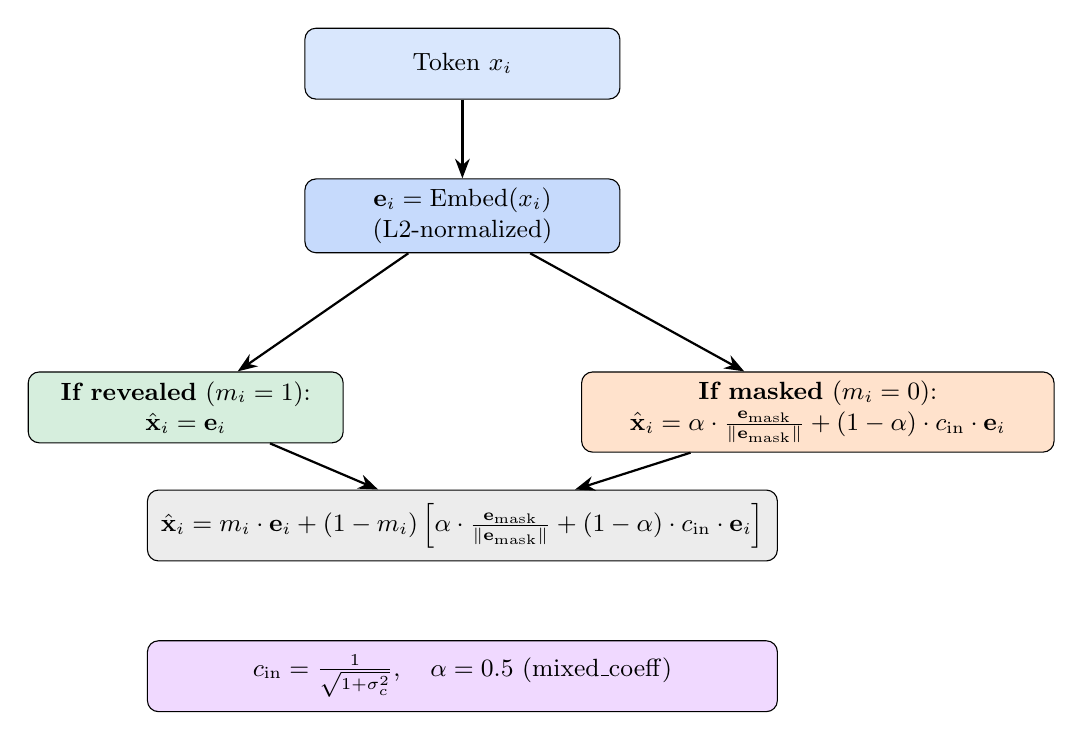
\begin{tikzpicture}[
    block/.style={draw, rounded corners, minimum width=4cm, minimum height=0.9cm, align=center, font=\small},
    arrow/.style={-{Stealth[length=2.5mm]}, thick},
    node distance=1.0cm
]
    % Token input
    \node[block, fill=embed!20] (tok) {Token $x_i$};
    \node[block, fill=embed!30, below=of tok] (emb) {$\mathbf{e}_i = \text{Embed}(x_i)$\\(L2-normalized)};
    
    % Branch
    \node[block, fill=norm!20, below left=1.5cm and -0.5cm of emb] (revealed) {\textbf{If revealed} ($m_i = 1$):\\$\hat{\mathbf{x}}_i = \mathbf{e}_i$};
    \node[block, fill=mask!20, below right=1.5cm and -0.5cm of emb, minimum width=6cm] (masked) {\textbf{If masked} ($m_i = 0$):\\$\hat{\mathbf{x}}_i = \alpha \cdot \frac{\mathbf{e}_{\text{mask}}}{\|\mathbf{e}_{\text{mask}}\|} + (1-\alpha) \cdot c_{\text{in}} \cdot \mathbf{e}_i$};
    
    % Merge
    \node[block, fill=gray!15, below=3cm of emb, minimum width=8cm] (merge) {$\hat{\mathbf{x}}_i = m_i \cdot \mathbf{e}_i + (1 - m_i)\left[\alpha \cdot \frac{\mathbf{e}_{\text{mask}}}{\|\mathbf{e}_{\text{mask}}\|} + (1-\alpha) \cdot c_{\text{in}} \cdot \mathbf{e}_i\right]$};
    
    % Parameters
    \node[block, fill=cond!15, below=of merge, minimum width=8cm] (params) {$c_{\text{in}} = \frac{1}{\sqrt{1 + \sigma_c^2}}, \quad \alpha = 0.5$ (mixed\_coeff)};
    
    \draw[arrow] (tok) -- (emb);
    \draw[arrow] (emb) -- (revealed);
    \draw[arrow] (emb) -- (masked);
    \draw[arrow] (revealed) -- (merge);
    \draw[arrow] (masked) -- (merge);
\end{tikzpicture}
\end{center}

\subsection{Timestep Conditioning in ContDIT}

The discrete noise probability $\alpha_d$ is converted to a log-scale sigma before being passed to the same \texttt{TimestepEmbedder}:
\[
\sigma_{\text{discrete}} = -\log(1 - \alpha_d)
\]
\[
\mathbf{c} = \text{SiLU}\!\left(\text{TimestepEmbedder}(\sigma_{\text{discrete}})\right) \in \mathbb{R}^{d_{\text{cond}}}
\]

\newpage

%% ============================================================
%% SECTION 4: FULL MATHEMATICAL DETAIL
%% ============================================================
\section{Level 3: Full Mathematical Detail}

\subsection{Embedding Layer}

\subsubsection{DDiT (dit.py)}
Standard learned embedding with Kaiming initialization:
\[
\mathbf{E} \in \mathbb{R}^{V \times d}, \quad \mathbf{e}_i = \mathbf{E}[x_i]
\]
For soft inputs (probability distributions over vocab):
\[
\mathbf{e} = \text{softmax}(\mathbf{p}) \cdot \mathbf{E}
\]

\subsubsection{ContDIT (dit\_cont.py)}
L2-normalized embedding (unit norm per token):
\[
\hat{\mathbf{E}}[i] = \frac{\mathbf{E}[i]}{\|\mathbf{E}[i]\|_2}, \quad i \in \{0, \ldots, V{-}2\}
\]
Note: only the first $V{-}1$ rows are normalized (mask token excluded from normalization in this variant).

\subsection{Timestep Embedder}

Sinusoidal positional encoding followed by a 2-layer MLP:
\[
\text{freq}_k = \exp\!\left(-\frac{\log(10000) \cdot k}{D/2}\right), \quad k = 0, \ldots, \frac{D}{2}-1
\]
\[
\mathbf{t}_{\text{freq}} = \left[\cos(t \cdot \text{freq}_0), \ldots, \cos(t \cdot \text{freq}_{D/2-1}),\; \sin(t \cdot \text{freq}_0), \ldots, \sin(t \cdot \text{freq}_{D/2-1})\right]
\]
\[
\mathbf{t}_{\text{emb}} = W_2 \cdot \text{SiLU}(W_1 \cdot \mathbf{t}_{\text{freq}} + b_1) + b_2 \in \mathbb{R}^{d_{\text{cond}}}
\]

In the main forward pass, an additional SiLU activation is applied:
\[
\mathbf{c} = \text{SiLU}(\mathbf{t}_{\text{emb}})
\]

\subsection{Rotary Position Embeddings (RoPE)}

For position $p$ and dimension pair $(2k, 2k{+}1)$:
\[
\text{RoPE}(\mathbf{q}, p)_{2k} = q_{2k} \cos(p \cdot \theta_k) - q_{2k+1} \sin(p \cdot \theta_k)
\]
\[
\text{RoPE}(\mathbf{q}, p)_{2k+1} = q_{2k} \sin(p \cdot \theta_k) + q_{2k+1} \cos(p \cdot \theta_k)
\]
where $\theta_k = 10000^{-2k/d_{\text{head}}}$.

Applied to Q and K only (V is unchanged).

\subsection{Layer Normalization}

Custom implementation (cast to float32 for numerical stability):
\[
\text{LayerNorm}(\mathbf{x}) = \gamma \odot \frac{\mathbf{x} - \mu}{\sqrt{\sigma^2 + \epsilon}}
\]
where $\gamma$ is a learnable weight (no bias), and the normalization is computed in float32.

\subsection{Adaptive Layer Normalization (adaLN)}

The conditioning vector $\mathbf{c}$ is projected to 6 modulation parameters per block:
\[
(\beta_1, \gamma_1, g_1, \beta_2, \gamma_2, g_2) = \text{Linear}(\mathbf{c}) \in \mathbb{R}^{6d}
\]
Initialized to zero (identity at start of training).

The modulation function:
\[
\text{Modulate}(\mathbf{x}, \beta, \gamma) = \mathbf{x} \odot (1 + \gamma) + \beta
\]

\subsection{DDiT Block --- Full Math}

Given input $\mathbf{x} \in \mathbb{R}^{B \times L \times d}$ and conditioning $\mathbf{c} \in \mathbb{R}^{B \times d_\text{cond}}$:

\begin{enumerate}
    \item \textbf{Save residual:} $\mathbf{x}_{\text{skip}} = \mathbf{x}$
    
    \item \textbf{Pre-norm + modulate (attention):}
    \[
    \mathbf{x}' = \text{Modulate}\!\left(\text{LayerNorm}(\mathbf{x}),\; \beta_1,\; \gamma_1\right)
    \]
    
    \item \textbf{QKV projection:}
    \[
    [\mathbf{Q}, \mathbf{K}, \mathbf{V}] = \mathbf{x}' W_{\text{qkv}} \in \mathbb{R}^{B \times L \times 3d}
    \]
    Reshaped to $B \times L \times H \times d_h$ per head.
    
    \item \textbf{RoPE:} Apply rotary embeddings to Q and K.
    
    \item \textbf{Scaled dot-product attention} (bidirectional, no mask):
    \[
    \text{Attn}(\mathbf{Q}, \mathbf{K}, \mathbf{V}) = \text{softmax}\!\left(\frac{\mathbf{Q}\mathbf{K}^\top}{\sqrt{d_h}}\right) \mathbf{V}
    \]
    
    \item \textbf{Output projection + gated residual:}
    \[
    \mathbf{x} = \mathbf{x}_{\text{skip}} + g_1 \odot \text{Dropout}\!\left(W_{\text{out}} \cdot \text{Attn}(\ldots)\right)
    \]
    
    \item \textbf{Pre-norm + modulate (MLP):}
    \[
    \mathbf{x}' = \text{Modulate}\!\left(\text{LayerNorm}(\mathbf{x}),\; \beta_2,\; \gamma_2\right)
    \]
    
    \item \textbf{MLP:}
    \[
    \text{MLP}(\mathbf{x}') = W_2 \cdot \text{GELU}_{\text{tanh}}(W_1 \mathbf{x}' + b_1) + b_2
    \]
    where $W_1 \in \mathbb{R}^{4d \times d}$, $W_2 \in \mathbb{R}^{d \times 4d}$.
    
    \item \textbf{Gated residual:}
    \[
    \mathbf{x} = \mathbf{x} + g_2 \odot \text{Dropout}\!\left(\text{MLP}(\mathbf{x}')\right)
    \]
\end{enumerate}

\subsection{Final Output Layer (DDiTFinalLayer)}

\begin{enumerate}
    \item \textbf{LayerNorm:} $\mathbf{x}' = \text{LayerNorm}(\mathbf{x})$
    \item \textbf{adaLN modulation} (2 parameters):
    \[
    (\beta_f, \gamma_f) = \text{Linear}(\mathbf{c}) \in \mathbb{R}^{2d}
    \]
    \[
    \mathbf{x}'' = \mathbf{x}' \odot (1 + \gamma_f) + \beta_f
    \]
    \item \textbf{Linear projection to logits:}
    \[
    \text{logits} = W_{\text{out}} \mathbf{x}'' + b_{\text{out}} \in \mathbb{R}^{B \times L \times V}
    \]
    Initialized to zero (model starts as identity).
\end{enumerate}

\newpage

%% ============================================================
%% SECTION 5: CONTDIT FULL FORWARD PASS
%% ============================================================
\section{Level 3: ContDIT Full Forward Pass}

\subsection{Complete Forward Pass Algorithm}

\noindent\textbf{Inputs:}
\begin{itemize}
    \item $\mathbf{x}_t \in \mathbb{Z}^{B \times L}$ --- corrupted token IDs
    \item $\alpha_d \in [0,1]^B$ --- discrete noise level (masking probability)
    \item $\sigma_c \in \mathbb{R}_+^B$ --- continuous noise standard deviation
    \item $\mathbf{m} \in \{0,1\}^{B \times L}$ --- reveal mask (1 = clean, 0 = still masked)
    \item (optional) $\tilde{\mathbf{E}} \in \mathbb{R}^{B \times L \times d}$ --- pre-computed noisy embeddings
\end{itemize}

\noindent\textbf{Step 1: Compute scaling factors}
\[
\sigma_{\text{disc}} = -\log(1 - \alpha_d) \in \mathbb{R}^B
\]
\[
c_{\text{in}} = \frac{1}{\sqrt{1 + \sigma_c^2}} \in \mathbb{R}^B
\]

\noindent\textbf{Step 2: Token embedding} (L2-normalized)
\[
\mathbf{e}_i = \frac{\mathbf{E}[x_{t,i}]}{\|\mathbf{E}[x_{t,i}]\|_2} \in \mathbb{R}^d
\]

\noindent\textbf{Step 3: Mask embedding} (normalized, from last row of $\mathbf{E}$)
\[
\mathbf{e}_{\text{mask}} = \frac{\mathbf{E}[V]}{\|\mathbf{E}[V]\|_2} \in \mathbb{R}^d
\]
(broadcast to $B \times L \times d$)

\noindent\textbf{Step 4: Hybrid input construction}
\[
\hat{\mathbf{x}}_i = m_i \cdot \mathbf{e}_i + (1 - m_i) \cdot \left[\alpha \cdot \mathbf{e}_{\text{mask}} + (1 - \alpha) \cdot c_{\text{in}} \cdot \mathbf{e}_i\right]
\]
where $\alpha = 0.5$ is the \texttt{mixed\_coeff} hyperparameter.

If external noisy embeddings $\tilde{\mathbf{E}}$ are provided:
\[
\hat{\mathbf{x}}_i = m_i \cdot \mathbf{e}_i + (1 - m_i) \cdot \left[\alpha \cdot \mathbf{e}_{\text{mask}} + (1 - \alpha) \cdot c_{\text{in}} \cdot \tilde{\mathbf{E}}_i\right]
\]

\noindent\textbf{Step 5: Timestep conditioning}
\[
\mathbf{c} = \text{SiLU}\!\left(\text{TimestepEmbedder}(\sigma_{\text{disc}})\right) \in \mathbb{R}^{B \times d_{\text{cond}}}
\]

\noindent\textbf{Step 6: Rotary embeddings}
\[
(\cos\Theta, \sin\Theta) = \text{Rotary}(\hat{\mathbf{x}})
\]

\noindent\textbf{Step 7: Transformer blocks} (in bfloat16)
\[
\hat{\mathbf{x}} \leftarrow \text{DDiTBlock}_i(\hat{\mathbf{x}}, (\cos\Theta, \sin\Theta), \mathbf{c}), \quad i = 1, \ldots, N
\]

\noindent\textbf{Step 8: Final layer}
\[
\text{logits} = \text{DDiTFinalLayer}(\hat{\mathbf{x}}, \mathbf{c}) \in \mathbb{R}^{B \times L \times V}
\]

\noindent\textbf{Step 9: Exclude mask token}
\[
\text{output} = \text{logits}[:, :, :V{-}1] \in \mathbb{R}^{B \times L \times (V{-}1)}
\]

\newpage

%% ============================================================
%% SECTION 6: DETAILED COMPONENT DIAGRAMS
%% ============================================================
\section{Level 3: Detailed Component Diagrams}

\subsection{Attention Mechanism Detail}

\begin{center}
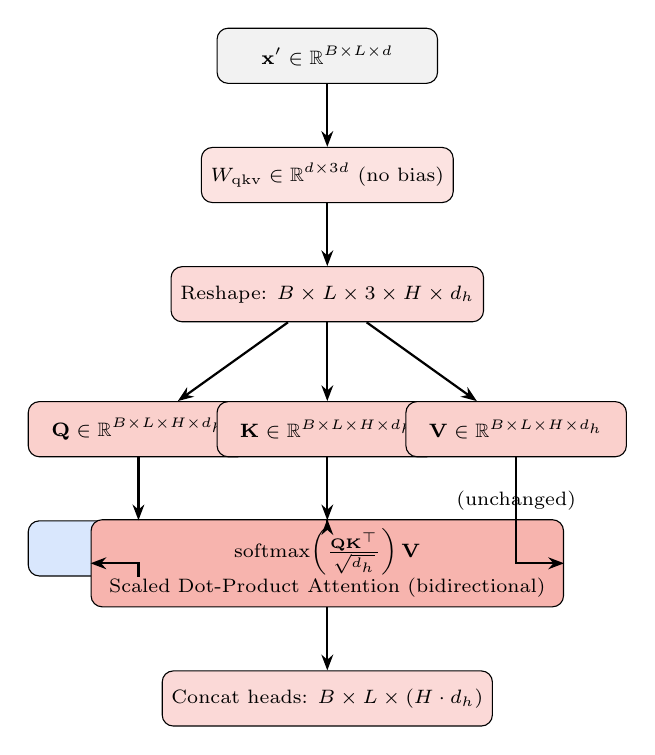
\begin{tikzpicture}[
    block/.style={draw, rounded corners, minimum width=2.8cm, minimum height=0.7cm, align=center, font=\scriptsize},
    arrow/.style={-{Stealth[length=2mm]}, thick},
    node distance=0.8cm
]
    % Input
    \node[block, fill=gray!10] (xin) {$\mathbf{x}' \in \mathbb{R}^{B \times L \times d}$};
    
    % QKV Linear
    \node[block, fill=attn!15, below=of xin] (wqkv) {$W_{\text{qkv}} \in \mathbb{R}^{d \times 3d}$ (no bias)};
    
    % Reshape
    \node[block, fill=attn!20, below=of wqkv] (reshape) {Reshape: $B \times L \times 3 \times H \times d_h$};
    
    % Split
    \node[block, fill=attn!25, below left=1cm and -1cm of reshape] (q) {$\mathbf{Q} \in \mathbb{R}^{B \times L \times H \times d_h}$};
    \node[block, fill=attn!25, below=1cm of reshape] (k) {$\mathbf{K} \in \mathbb{R}^{B \times L \times H \times d_h}$};
    \node[block, fill=attn!25, below right=1cm and -1cm of reshape] (v) {$\mathbf{V} \in \mathbb{R}^{B \times L \times H \times d_h}$};
    
    % RoPE
    \node[block, fill=embed!20, below=of q] (ropeq) {RoPE($\mathbf{Q}$)};
    \node[block, fill=embed!20, below=of k] (ropek) {RoPE($\mathbf{K}$)};
    \node[font=\scriptsize, below=0.3cm of v] (noop) {(unchanged)};
    
    % SDPA
    \node[block, fill=attn!40, below=2.5cm of reshape, minimum width=6cm] (sdpa) {$\text{softmax}\!\left(\frac{\mathbf{Q}\mathbf{K}^\top}{\sqrt{d_h}}\right)\mathbf{V}$\\Scaled Dot-Product Attention (bidirectional)};
    
    % Concat heads
    \node[block, fill=attn!20, below=of sdpa] (concat) {Concat heads: $B \times L \times (H \cdot d_h)$};
    
    \draw[arrow] (xin) -- (wqkv);
    \draw[arrow] (wqkv) -- (reshape);
    \draw[arrow] (reshape) -- (q);
    \draw[arrow] (reshape) -- (k);
    \draw[arrow] (reshape) -- (v);
    \draw[arrow] (q) -- (ropeq);
    \draw[arrow] (k) -- (ropek);
    \draw[arrow] (ropeq) |- (sdpa);
    \draw[arrow] (ropek) -- (sdpa);
    \draw[arrow] (v) |- (sdpa);
    \draw[arrow] (sdpa) -- (concat);
\end{tikzpicture}
\end{center}

\subsection{MLP Detail}

\begin{center}
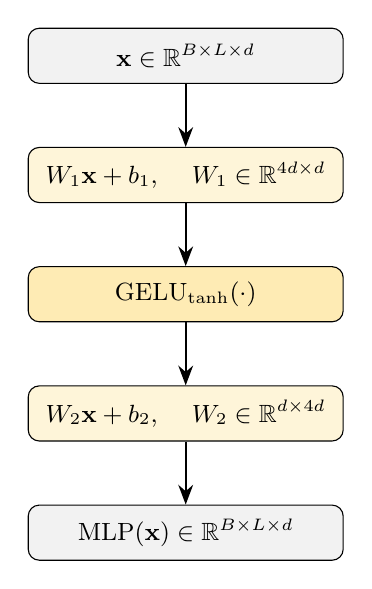
\begin{tikzpicture}[
    block/.style={draw, rounded corners, minimum width=4cm, minimum height=0.7cm, align=center, font=\small},
    arrow/.style={-{Stealth[length=2.5mm]}, thick},
    node distance=0.8cm
]
    \node[block, fill=gray!10] (in) {$\mathbf{x} \in \mathbb{R}^{B \times L \times d}$};
    \node[block, fill=mlp!15, below=of in] (w1) {$W_1 \mathbf{x} + b_1$, \quad $W_1 \in \mathbb{R}^{4d \times d}$};
    \node[block, fill=mlp!30, below=of w1] (gelu) {$\text{GELU}_{\text{tanh}}(\cdot)$};
    \node[block, fill=mlp!15, below=of gelu] (w2) {$W_2 \mathbf{x} + b_2$, \quad $W_2 \in \mathbb{R}^{d \times 4d}$};
    \node[block, fill=gray!10, below=of w2] (out) {$\text{MLP}(\mathbf{x}) \in \mathbb{R}^{B \times L \times d}$};
    
    \draw[arrow] (in) -- (w1);
    \draw[arrow] (w1) -- (gelu);
    \draw[arrow] (gelu) -- (w2);
    \draw[arrow] (w2) -- (out);
\end{tikzpicture}
\end{center}

where:
\[
\text{GELU}_{\text{tanh}}(x) = 0.5\, x \left(1 + \tanh\!\left[\sqrt{2/\pi}\,(x + 0.044715\, x^3)\right]\right)
\]

\subsection{Bias-Dropout-Scale Residual Connection}

The fused kernel computes:
\[
\text{BiasDropoutScale}(\mathbf{x}, \text{bias}, \text{scale}, \mathbf{x}_{\text{skip}}, p) = \mathbf{x}_{\text{skip}} + \text{scale} \odot \text{Dropout}(\mathbf{x} + \text{bias},\; p)
\]

In adaLN mode, the ``scale'' is the \textbf{gate} parameter $g \in \mathbb{R}^d$ from the conditioning.

\newpage

%% ============================================================
%% SECTION 7: SIDE-BY-SIDE COMPARISON
%% ============================================================
\section{Summary: DDiT vs ContDIT Comparison}

\begin{center}
\renewcommand{\arraystretch}{1.4}
\begin{tabular}{@{}p{3.5cm}p{5cm}p{5.5cm}@{}}
\toprule
\textbf{Component} & \textbf{DDiT} & \textbf{ContDIT} \\
\midrule
\textbf{Algorithm} & MDLM / SEDD (pure discrete) & CANDI (hybrid discrete + continuous) \\
\textbf{Input tokens} & $\mathbf{x} \in \mathbb{Z}^{B \times L}$ & $\mathbf{x}_t \in \mathbb{Z}^{B \times L}$ \\
\textbf{Noise inputs} & $\sigma \in \mathbb{R}^B$ (scalar) & $\alpha_d$, $\sigma_c$, reveal mask $\mathbf{m}$ \\
\textbf{Embedding} & $\mathbf{E}[x]$ (standard) & $\mathbf{E}[x] / \|\mathbf{E}[x]\|_2$ (L2-normalized) \\
\textbf{Input construction} & Direct embedding lookup & Hybrid blend of mask emb + scaled token emb \\
\textbf{Timestep $\sigma$} & Passed directly & $\sigma = -\log(1 - \alpha_d)$ \\
\textbf{Continuous scaling} & N/A & $c_{\text{in}} = 1/\sqrt{1+\sigma_c^2}$ \\
\textbf{Transformer blocks} & DDiTBlock (adaLN + RoPE + MLP) & Same DDiTBlock \\
\textbf{Output dim} & $V$ (full vocab) & $V - 1$ (mask token excluded) \\
\textbf{Initialization} & adaLN \& final layer $\to$ zero & Same \\
\bottomrule
\end{tabular}
\end{center}

%% ============================================================
%% SECTION 8: FULL DATA FLOW DIAGRAM
%% ============================================================
\section{Complete Data Flow: ContDIT End-to-End}

\begin{center}
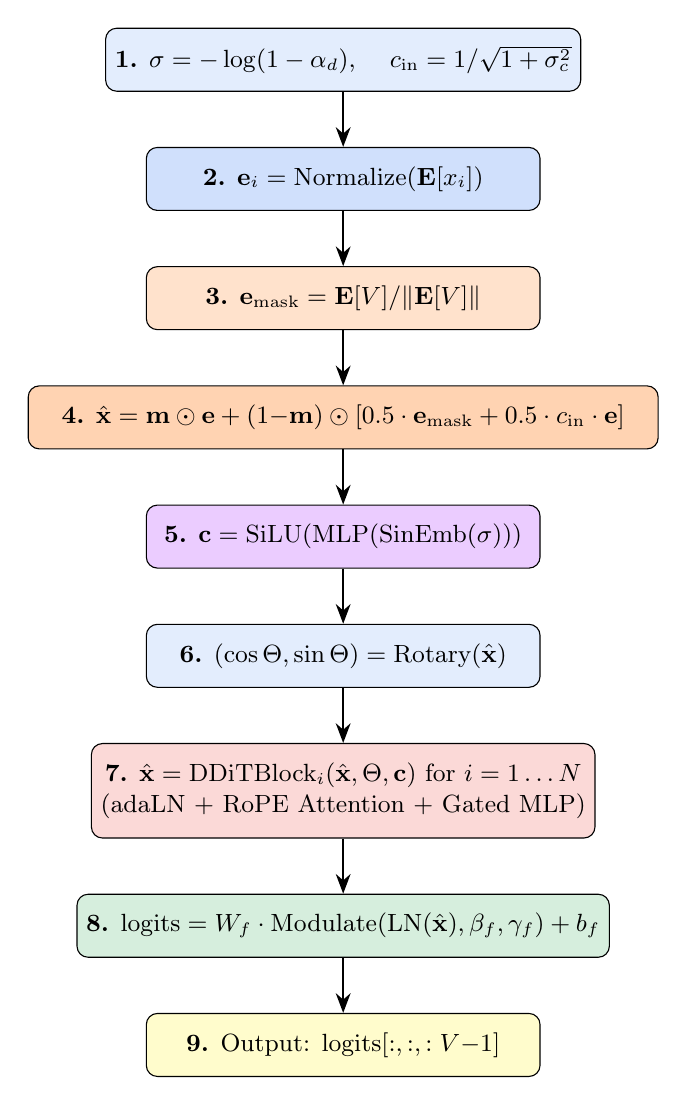
\begin{tikzpicture}[
    block/.style={draw, rounded corners, minimum width=5cm, minimum height=0.8cm, align=center, font=\small},
    smallblock/.style={draw, rounded corners, minimum width=3cm, minimum height=0.6cm, align=center, font=\scriptsize},
    arrow/.style={-{Stealth[length=2.5mm]}, thick},
    node distance=0.7cm
]
    \node[block, fill=embed!15] (s1) {\textbf{1.} $\sigma = -\log(1-\alpha_d)$, \quad $c_{\text{in}} = 1/\sqrt{1+\sigma_c^2}$};
    \node[block, fill=embed!25, below=of s1] (s2) {\textbf{2.} $\mathbf{e}_i = \text{Normalize}(\mathbf{E}[x_i])$};
    \node[block, fill=mask!20, below=of s2] (s3) {\textbf{3.} $\mathbf{e}_{\text{mask}} = \mathbf{E}[V] / \|\mathbf{E}[V]\|$};
    \node[block, fill=mask!30, below=of s3, minimum width=8cm] (s4) {\textbf{4.} $\hat{\mathbf{x}} = \mathbf{m} \odot \mathbf{e} + (1{-}\mathbf{m}) \odot [0.5 \cdot \mathbf{e}_{\text{mask}} + 0.5 \cdot c_{\text{in}} \cdot \mathbf{e}]$};
    \node[block, fill=cond!20, below=of s4] (s5) {\textbf{5.} $\mathbf{c} = \text{SiLU}(\text{MLP}(\text{SinEmb}(\sigma)))$};
    \node[block, fill=embed!15, below=of s5] (s6) {\textbf{6.} $(\cos\Theta, \sin\Theta) = \text{Rotary}(\hat{\mathbf{x}})$};
    \node[block, fill=attn!20, below=of s6, minimum height=1.2cm] (s7) {\textbf{7.} $\hat{\mathbf{x}} = \text{DDiTBlock}_i(\hat{\mathbf{x}}, \Theta, \mathbf{c})$ for $i=1\ldots N$\\(adaLN + RoPE Attention + Gated MLP)};
    \node[block, fill=norm!20, below=of s7] (s8) {\textbf{8.} $\text{logits} = W_f \cdot \text{Modulate}(\text{LN}(\hat{\mathbf{x}}), \beta_f, \gamma_f) + b_f$};
    \node[block, fill=yellow!20, below=of s8] (s9) {\textbf{9.} Output: $\text{logits}[:,:,:V{-}1]$};
    
    \draw[arrow] (s1) -- (s2);
    \draw[arrow] (s2) -- (s3);
    \draw[arrow] (s3) -- (s4);
    \draw[arrow] (s4) -- (s5);
    \draw[arrow] (s5) -- (s6);
    \draw[arrow] (s6) -- (s7);
    \draw[arrow] (s7) -- (s8);
    \draw[arrow] (s8) -- (s9);
\end{tikzpicture}
\end{center}

\newpage

%% ============================================================
%% SECTION 9: INITIALIZATION AND TRAINING NOTES
%% ============================================================
\section{Initialization and Implementation Notes}

\subsection{Zero Initialization Strategy}

Key layers are initialized to \textbf{zero} so the model starts as an identity function:
\begin{itemize}
    \item \texttt{adaLN\_modulation} (weight and bias) $\to 0$ in every DDiTBlock
    \item \texttt{DDiTFinalLayer.linear} (weight and bias) $\to 0$
    \item \texttt{DDiTFinalLayer.adaLN\_modulation} (weight and bias) $\to 0$
\end{itemize}
This means at initialization:
\begin{itemize}
    \item All gates $g_1, g_2 = 0$ $\Rightarrow$ residual connections are pure skip
    \item All shifts $\beta = 0$, scales $\gamma = 0$ $\Rightarrow$ modulation is identity
    \item Final projection outputs all zeros
\end{itemize}

\subsection{Precision and Numerical Stability}

\begin{itemize}
    \item \textbf{LayerNorm}: Cast to float32 internally for stability
    \item \textbf{RoPE}: Applied in float32 (autocast disabled)
    \item \textbf{Transformer blocks}: Run in bfloat16 via \texttt{torch.cuda.amp.autocast}
    \item \textbf{Embedding normalization} (ContDIT): Computed in float32
\end{itemize}

\subsection{Hyperparameters}

\begin{center}
\begin{tabular}{@{}lll@{}}
\toprule
\textbf{Parameter} & \textbf{Symbol} & \textbf{Typical Value} \\
\midrule
Hidden dimension & $d$ & \texttt{config.hidden\_size} \\
Conditioning dimension & $d_{\text{cond}}$ & \texttt{config.cond\_dim} \\
Number of heads & $H$ & \texttt{config.n\_heads} \\
Head dimension & $d_h = d/H$ & --- \\
Number of blocks & $N$ & \texttt{config.n\_blocks} \\
MLP ratio & --- & 4 \\
Dropout & $p$ & \texttt{config.dropout} \\
Mixed coefficient (ContDIT) & $\alpha$ & 0.5 \\
Frequency embedding dim & $D$ & 256 \\
RoPE base & --- & 10{,}000 \\
\bottomrule
\end{tabular}
\end{center}

\end{document}
